% Five ways to write better Python, COMP64803 talk (about 10 minutes).
% Standard Beamer theme (Madrid). Compile with pdfLaTeX on Overleaf.
% Every figure is drawn with TikZ, so the project is this single file.
\documentclass[aspectratio=169,11pt]{beamer}
\usetheme{Madrid}
\setbeamertemplate{navigation symbols}{}
\setbeamerfont{block body}{size=\small}

\usepackage[T1]{fontenc}
\usepackage[utf8]{inputenc}
\usepackage{lmodern}
\usepackage{amsmath,amssymb}
\usepackage{listings}
\usepackage{tikz}
\usetikzlibrary{arrows.meta,positioning,calc}

% Colours of the figures, taken from the Beamer palette
\definecolor{fast}{rgb}{0.2,0.2,0.7}
\colorlet{slow}{red!75!black}

% Tighter space around displayed formulas inside blocks
\addtobeamertemplate{block begin}{}{%
  \setlength{\abovedisplayskip}{3pt}\setlength{\abovedisplayshortskip}{1pt}%
  \setlength{\belowdisplayskip}{3pt}\setlength{\belowdisplayshortskip}{3pt}}

% Python listings, with !!...!! marking the part that makes the code fast
\lstset{
  language=Python,
  basicstyle=\ttfamily\fontsize{8.3}{10}\selectfont,
  keywordstyle=\color{fast}\bfseries,
  commentstyle=\color{gray},
  stringstyle=\color{slow},
  showstringspaces=false,
  columns=fixed,
  basewidth=0.53em,
  keepspaces=true,
  upquote=true,
  frame=single, rulecolor=\color{gray!50}, framesep=4pt,
  xleftmargin=4pt, xrightmargin=4pt,
  aboveskip=0pt, belowskip=0pt,
  moredelim=[is][\bfseries\color{fast}]{!!}{!!},
}

\tikzset{
  cell/.style={draw, minimum width=0.65cm, minimum height=0.55cm, inner sep=0pt, font=\small},
  lbl/.style={font=\footnotesize, anchor=west},
}

\title[Five ways to write better Python]{Five ways to write better Python}
\author[H. Eljabiri]{Hamza Eljabiri}
\institute[Manchester]{COMP64803 Introduction to Responsible and Reproducible AI\\
  The University of Manchester}
\date{November 2026}

\begin{document}

% ================================================================ title
\begin{frame}
  \titlepage
\end{frame}

% ================================================================ 1. sets
\begin{frame}{Sets for membership tests}
  \begin{columns}[T,onlytextwidth]
  \begin{column}{0.55\textwidth}
    \vspace{4mm}
    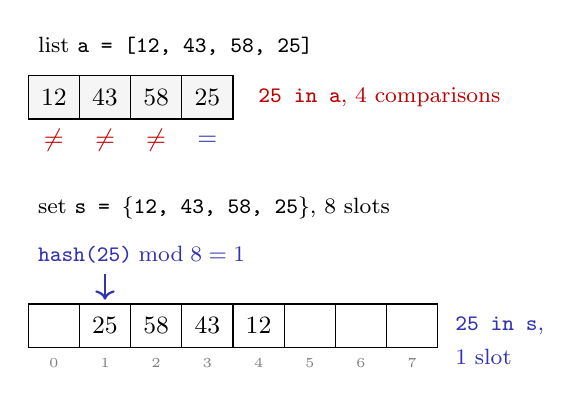
\begin{tikzpicture}
      \node[lbl] at (0,1.6) {list \texttt{a = [12, 43, 58, 25]}};
      \foreach \v [count=\i from 0] in {12,43,58,25}
        \node[cell, fill=gray!8] at (\i*0.65+0.325,0.95) {\v};
      \foreach \i in {0,1,2}
        \node[font=\small, slow] at (\i*0.65+0.325,0.4) {$\neq$};
      \node[font=\small, fast] at (3*0.65+0.325,0.4) {$=$};
      \node[lbl, slow] at (2.8,0.95) {\texttt{25 in a}, 4 comparisons};
      \node[lbl] at (0,-0.45) {set \texttt{s = \{12, 43, 58, 25\}}, 8 slots};
      \node[font=\footnotesize, fast, anchor=west] at (0,-1.05) {$\texttt{hash(25)} \bmod 8 = 1$};
      \draw[->, fast, thick] (0.975,-1.3) -- (0.975,-1.62);
      \foreach \v [count=\i from 0] in {{},25,58,43,12,{},{},{}}
        \node[cell] at (\i*0.65+0.325,-1.95) {\v};
      \foreach \i in {0,...,7}
        \node[font=\tiny, gray] at (\i*0.65+0.325,-2.42) {\i};
      \node[lbl, fast] at (5.3,-1.95) {\texttt{25 in s},};
      \node[lbl, fast] at (5.3,-2.35) {1 slot};
    \end{tikzpicture}
  \end{column}
  \begin{column}{0.42\textwidth}
    \begin{block}{List}
      \texttt{x in a\_list} compares $x$ with the elements one by one.
      \[ T(n) = O(n) \]
    \end{block}
    \begin{block}{Set}
      \texttt{x in a\_set} looks only in the slot given by \texttt{hash(x)}.
      \[ T(n) = O(1) \ \text{on average} \]
    \end{block}
    \begin{block}{Price}
      Building the set costs $O(n)$ once, and its elements must be hashable.
    \end{block}
  \end{column}
  \end{columns}
\end{frame}

\begin{frame}[fragile]{Sets in code}
  \begin{columns}[T,onlytextwidth]
  \begin{column}{0.60\textwidth}
\begin{lstlisting}
def count_hits(items, queries):
    return sum(1 for q in queries if q in items)

ids = list(range(100_000))
ids_set = !!set(ids)!!                # built once
queries = range(0, 200_000, 200)  # 1,000 queries

count_hits(ids, queries)      # 500
count_hits(ids_set, queries)  # 500
\end{lstlisting}
  \end{column}
  \begin{column}{0.37\textwidth}
    \begin{block}{Measurement}
      1,000 lookups among 100,000 ids\par\smallskip
      \begin{tabular}{@{}ll@{}}
        list & 319 ms\\
        set & \textbf{0.11 ms}\\
      \end{tabular}\par\smallskip
      about 2,900 times faster
    \end{block}
    \begin{block}{Dictionaries}
      The keys of a \texttt{dict} sit in the same kind of table, so \texttt{key in d} and
      \texttt{d[key]} also take $O(1)$ on average.
    \end{block}
  \end{column}
  \end{columns}
\end{frame}

% ================================================================ 2. deques
\begin{frame}{Deques for queues}
  \begin{columns}[T,onlytextwidth]
  \begin{column}{0.55\textwidth}
    \vspace{4mm}
    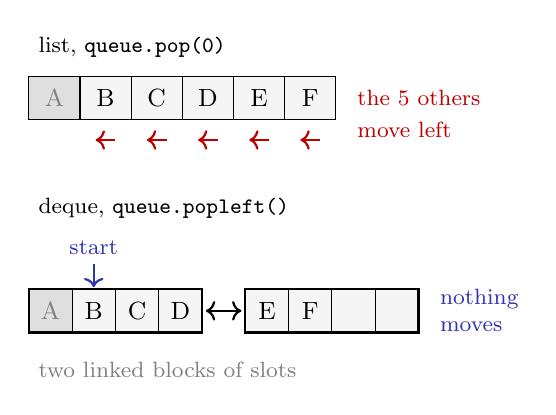
\begin{tikzpicture}
      \node[lbl] at (0,1.6) {list, \texttt{queue.pop(0)}};
      \node[cell, fill=gray!25, text=gray] at (0.325,0.95) {A};
      \foreach \v [count=\i from 1] in {B,C,D,E,F}
        \node[cell, fill=gray!8] at (\i*0.65+0.325,0.95) {\v};
      \foreach \i in {1,...,5}
        \draw[->, slow, thick] (\i*0.65+0.45,0.42) -- (\i*0.65+0.2,0.42);
      \node[lbl, slow] at (4.05,0.95) {the 5 others};
      \node[lbl, slow] at (4.05,0.55) {move left};
      \node[lbl] at (0,-0.45) {deque, \texttt{queue.popleft()}};
      \node[font=\footnotesize, fast] at (0.825,-0.95) {start};
      \draw[->, fast, thick] (0.825,-1.15) -- (0.825,-1.45);
      \node[cell, fill=gray!25, text=gray, minimum width=0.55cm] at (0.275,-1.75) {A};
      \foreach \v [count=\i from 1] in {B,C,D}
        \node[cell, fill=gray!8, minimum width=0.55cm] at (\i*0.55+0.275,-1.75) {\v};
      \draw[thick] (0,-2.025) rectangle (2.2,-1.475);
      \foreach \v [count=\i from 0] in {E,F,{},{}}
        \node[cell, fill=gray!8, minimum width=0.55cm] at (\i*0.55+3.025,-1.75) {\v};
      \draw[thick] (2.75,-2.025) rectangle (4.95,-1.475);
      \draw[<->, thick] (2.25,-1.75) -- (2.7,-1.75);
      \node[lbl, fast] at (5.1,-1.6) {nothing};
      \node[lbl, fast] at (5.1,-1.95) {moves};
      \node[lbl, gray] at (0,-2.5) {two linked blocks of slots};
    \end{tikzpicture}
  \end{column}
  \begin{column}{0.42\textwidth}
    \begin{block}{List}
      Serving $n$ customers with \texttt{pop(0)} moves
      \[ \sum_{k=1}^{n-1} k = \frac{n(n-1)}{2} \ \text{items}, \quad T(n) = O(n^2). \]
    \end{block}
    \begin{block}{Deque}
      \texttt{popleft()} only moves the start of the queue.
      \[ T(n) = O(n) \]
    \end{block}
    \begin{block}{Doubling}
      Doubling $n$ multiplies the list time by 4 and the deque time by 2.
    \end{block}
  \end{column}
  \end{columns}
\end{frame}

\begin{frame}[fragile]{Deques in code}
  \begin{columns}[T,onlytextwidth]
  \begin{column}{0.60\textwidth}
\begin{lstlisting}
from collections import deque

def serve_with_list(n):
    queue = list(range(n))
    return [queue.pop(0) for _ in range(n)]

def serve_with_deque(n):
    queue = !!deque(range(n))!!
    return [!!queue.popleft()!! for _ in range(n)]

serve_with_deque(5)   # [0, 1, 2, 3, 4]
\end{lstlisting}
  \end{column}
  \begin{column}{0.37\textwidth}
    \begin{block}{Measurement}
      50,000 customers\par\smallskip
      \begin{tabular}{@{}ll@{}}
        list & 181 ms\\
        deque & \textbf{2.05 ms}\\
      \end{tabular}\par\smallskip
      about 90 times faster, and the gap grows with $n$
    \end{block}
    \begin{block}{Indexing}
      \texttt{d[i]} in the middle of a deque costs $O(n)$, so a list is better for indexing.
    \end{block}
  \end{column}
  \end{columns}
\end{frame}

% ================================================================ 3. generators
\begin{frame}{Generators for single-pass loops}
  \begin{columns}[T,onlytextwidth]
  \begin{column}{0.55\textwidth}
    \vspace{4mm}
    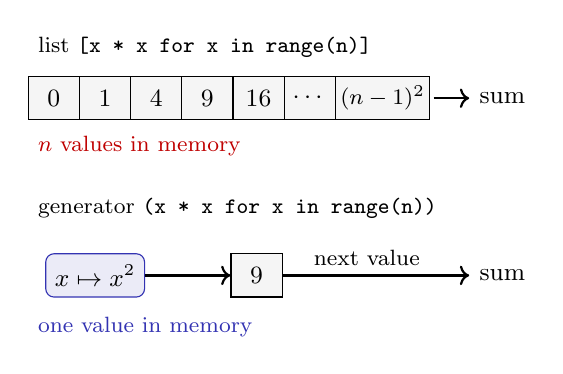
\begin{tikzpicture}
      \node[lbl] at (0,1.6) {list \texttt{[x * x for x in range(n)]}};
      \foreach \v [count=\i from 0] in {0,1,4,9,16}
        \node[cell, fill=gray!8] at (\i*0.65+0.325,0.95) {\v};
      \node[cell, fill=gray!8] at (3.575,0.95) {$\cdots$};
      \node[cell, fill=gray!8, minimum width=1.2cm, font=\footnotesize] at (4.5,0.95) {$(n-1)^2$};
      \draw[->, thick] (5.15,0.95) -- (5.6,0.95) node[right, font=\small] {sum};
      \node[lbl, slow] at (0,0.35) {$n$ values in memory};
      \node[lbl] at (0,-0.45) {generator \texttt{(x * x for x in range(n))}};
      \node[draw=fast, fill=fast!10, rounded corners=3pt, font=\small, minimum height=0.55cm]
        (g) at (0.85,-1.3) {$x \mapsto x^2$};
      \node[cell, fill=gray!8] (v) at (2.9,-1.3) {9};
      \draw[->, thick] (g) -- (v);
      \draw[->, thick] (v) -- (5.6,-1.3) node[right, font=\small] {sum};
      \node[font=\footnotesize, anchor=south] at (4.3,-1.3) {next value};
      \node[lbl, fast] at (0,-1.95) {one value in memory};
    \end{tikzpicture}
  \end{column}
  \begin{column}{0.42\textwidth}
    \begin{block}{List comprehension}
      Builds all $n$ values before \texttt{sum} starts. Memory $O(n)$.
    \end{block}
    \begin{block}{Generator expression}
      Computes the next value when \texttt{sum} asks for it. Memory $O(1)$.
    \end{block}
    \begin{block}{Same result}
      \[ \sum_{x=0}^{n-1} x^2 = \frac{(n-1)\,n\,(2n-1)}{6} \]
    \end{block}
  \end{column}
  \end{columns}
\end{frame}

\begin{frame}[fragile]{Generators in code}
  \begin{columns}[T,onlytextwidth]
  \begin{column}{0.60\textwidth}
\begin{lstlisting}
def sum_with_list(n):
    return sum([x * x for x in range(n)])

def sum_with_generator(n):
    return sum(!!x * x for x in range(n)!!)

squares = (x * x for x in range(4))
sum(squares)   # 14
sum(squares)   # 0, already used up
\end{lstlisting}
  \end{column}
  \begin{column}{0.37\textwidth}
    \begin{block}{Measurement}
      Peak memory for $n = 1{,}000{,}000$\par\smallskip
      \begin{tabular}{@{}lr@{}}
        list & 40,448,200 bytes\\
        generator & \textbf{464 bytes}\\
      \end{tabular}
    \end{block}
    \begin{block}{One pass}
      A generator can be read once. A second pass, \texttt{len} or an index need a list.
    \end{block}
  \end{column}
  \end{columns}
\end{frame}

% ================================================================ 4. cache
\begin{frame}{Caching for repeated calls}
  \begin{columns}[T,onlytextwidth]
  \begin{column}{0.55\textwidth}
    \centering
    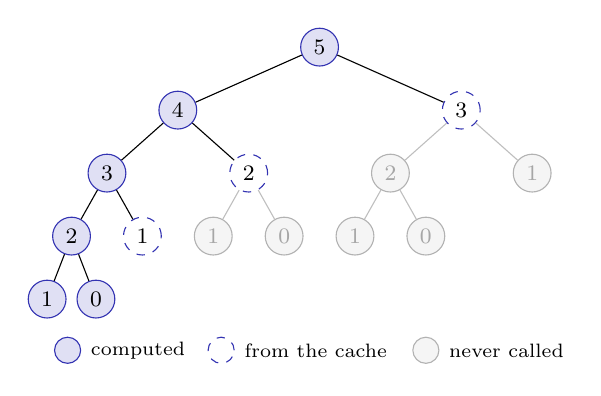
\begin{tikzpicture}[
      level distance=0.8cm,
      level 1/.style={sibling distance=3.6cm},
      level 2/.style={sibling distance=1.8cm},
      level 3/.style={sibling distance=0.9cm},
      level 4/.style={sibling distance=0.62cm},
      every node/.style={circle, inner sep=0pt, minimum size=0.48cm, font=\footnotesize},
      run/.style={draw=fast, fill=fast!15},
      hit/.style={draw=fast, dashed, fill=white},
      skip/.style={draw=gray!60, text=gray!70, fill=gray!8},
      dim/.style={edge from parent/.style={draw=gray!50}},
    ]
    \node[run] {5}
      child {node[run] {4}
        child {node[run] {3}
          child {node[run] {2}
            child {node[run] {1}}
            child {node[run] {0}}}
          child {node[hit] {1}}}
        child {node[hit] {2}
          child[dim] {node[skip] {1}}
          child[dim] {node[skip] {0}}}}
      child {node[hit] {3}
        child[dim] {node[skip] {2}
          child {node[skip] {1}}
          child {node[skip] {0}}}
        child[dim] {node[skip] {1}}};
    \begin{scope}[yshift=-3.85cm, every node/.style={font=\scriptsize}]
      \node[draw=fast, fill=fast!15, circle, minimum size=0.28cm] (a) at (-3.2,0) {};
      \node[anchor=west] at (a.east) {computed};
      \node[draw=fast, dashed, circle, minimum size=0.28cm] (b) at (-1.25,0) {};
      \node[anchor=west] at (b.east) {from the cache};
      \node[draw=gray!60, fill=gray!8, circle, minimum size=0.28cm] (c) at (1.35,0) {};
      \node[anchor=west] at (c.east) {never called};
    \end{scope}
    \end{tikzpicture}
  \end{column}
  \begin{column}{0.42\textwidth}
    \begin{block}{Plain recursion}
      Each call makes two more, $C(n) = 1 + C(n-1) + C(n-2)$, so
      \[ C(n) = 2F_{n+1} - 1, \]
      which is 2,692,537 calls for $n = 30$.
    \end{block}
    \begin{block}{With \texttt{@cache}}
      Each value is computed once. For $n = 30$, 31 values, and 28 calls read the cache.
    \end{block}
    \begin{block}{Condition}
      Same arguments give the same result, and the arguments are hashable.
    \end{block}
  \end{column}
  \end{columns}
\end{frame}

\begin{frame}[fragile]{Caching in code}
  \begin{columns}[T,onlytextwidth]
  \begin{column}{0.60\textwidth}
\begin{lstlisting}
from functools import cache

def fib(n):
    if n < 2:
        return n
    return fib(n - 1) + fib(n - 2)

!!@cache!!
def fib_cached(n):
    if n < 2:
        return n
    return fib_cached(n - 1) + fib_cached(n - 2)

fib_cached(30)            # 832040
fib_cached.cache_info()   # hits=28, misses=31
\end{lstlisting}
  \end{column}
  \begin{column}{0.37\textwidth}
    \begin{block}{Measurement}
      \texttt{fib(30)}\par\smallskip
      \begin{tabular}{@{}ll@{}}
        plain & 70 ms\\
        \texttt{@cache} & \textbf{0.013 ms}\\
      \end{tabular}\par\smallskip
      about 5,500 times faster
    \end{block}
    \begin{block}{Memory}
      \texttt{@cache} keeps every result, \texttt{@lru\_cache(maxsize=128)} only the 128 most
      recent ones.
    \end{block}
  \end{column}
  \end{columns}
\end{frame}

% ================================================================ 5. bisect
\begin{frame}{Binary search on sorted lists}
  \begin{columns}[T,onlytextwidth]
  \begin{column}{0.55\textwidth}
    \vspace{4mm}
    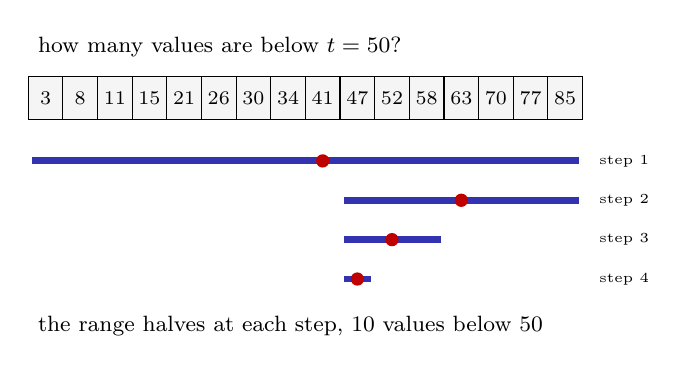
\begin{tikzpicture}[x=0.44cm]
      \node[lbl] at (0,1.15) {how many values are below $t = 50$?};
      \foreach \v [count=\i from 0] in {3,8,11,15,21,26,30,34,41,47,52,58,63,70,77,85}
        \node[cell, minimum width=0.44cm, font=\scriptsize, fill=gray!8] at (\i+0.5,0.5) {\v};
      \foreach \a/\b/\m/\yy/\s in {0/16/8/-0.3/1, 9/16/12/-0.8/2, 9/12/10/-1.3/3, 9/10/9/-1.8/4} {
        \draw[fast, line width=2.5pt] (\a+0.1,\yy) -- (\b-0.1,\yy);
        \fill[slow] (\m+0.5,\yy) circle (2.4pt);
        \node[font=\tiny, anchor=west] at (16.2,\yy) {step \s};
      }
      \node[lbl] at (0,-2.4) {the range halves at each step, 10 values below 50};
    \end{tikzpicture}
  \end{column}
  \begin{column}{0.42\textwidth}
    \begin{block}{Scan}
      Looking at every value takes $n$ comparisons.
    \end{block}
    \begin{block}{Bisection}
      Compare $t$ with the middle value and keep the half that holds the answer.
      \[ \lfloor \log_2 n \rfloor + 1 \ \text{comparisons at most} \]
      which is 17 for $n = 100{,}000$.
    \end{block}
    \begin{block}{Price}
      The list must be sorted, which costs $O(n \log n)$ once.
    \end{block}
  \end{column}
  \end{columns}
\end{frame}

\begin{frame}[fragile]{Binary search in code}
  \begin{columns}[T,onlytextwidth]
  \begin{column}{0.60\textwidth}
\begin{lstlisting}
import random
from bisect import bisect_left

def count_below(values, t):
    return sum(1 for v in values if v < t)

def count_below_sorted(sorted_values, t):
    return !!bisect_left(sorted_values, t)!!

rng = random.Random(0)
scores = sorted(rng.uniform(0, 100)
                for _ in range(100_000))
count_below_sorted(scores, 50)   # below 50
\end{lstlisting}
  \end{column}
  \begin{column}{0.37\textwidth}
    \begin{block}{Measurement}
      100 thresholds on 100,000 scores\par\smallskip
      \begin{tabular}{@{}ll@{}}
        scan & 301 ms\\
        bisect & \textbf{0.077 ms}\\
      \end{tabular}\par\smallskip
      about 3,900 times faster
    \end{block}
    \begin{block}{Left or right}
      \texttt{bisect\_left} counts the values $< t$, \texttt{bisect\_right} the values
      $\le t$.
    \end{block}
  \end{column}
  \end{columns}
\end{frame}

\end{document}
